%%%%%%%%%%%%%%%%%%%%%%%%%%%%%%%%%%%%%%%%%%%%%%%%%%%%%%%%%%%%%%%%%%%%%%%%%%%%%%%%%%%%%%%%%%%%%%%%%%%%%%%%%%%%%%%%%%%%%%%%%%%%%%%%%%%%%%%%%%%%%%%%%%%%%%%%%%%
% This is just an example/guide for you to refer to when submitting manuscripts to Frontiers, it is not mandatory to use Frontiers .cls files nor frontiers.tex  %
% This will only generate the Manuscript, the final article will be typeset by Frontiers after acceptance.   
%                                              %
%                                                                                                                                                         %
% When submitting your files, remember to upload this *tex file, the pdf generated with it, the *bib file (if bibliography is not\daleth  within the *tex) and all the figures.
%%%%%%%%%%%%%%%%%%%%%%%%%%%%%%%%%%%%%%%%%%%%%%%%%%%%%%%%%%%%%%%%%%%%%%%%%%%%%%%%%%%%%%%%%%%%%%%%%%%%%%%%%%%%%%%%%%%%%%%%%%%%%%%%%%%%%%%%%%%%%%%%%%%%%%%%%%%

%%% Version 3.4 Generated 2022/06/14 %%%
%%% You will need to have the following packages installed: datetime, fmtcount, etoolbox, fcprefix, which are normally inlcuded in WinEdt. %%%
%%% In http://www.ctan.org/ you can find the packages and how to install them, if necessary. %%%
%%%  NB logo1.jpg is required in the path in order to correctly compile front page header %%%

\documentclass[utf8]{FrontiersinVancouver} 
\usepackage{url,hyperref,lineno,microtype,subcaption,framed, float, dirtytalk, amsmath, tikz}
\usepackage[onehalfspacing]{setspace}

\linenumbers
% Leave a blank line between paragraphs instead of using \\ 


\def\keyFont{\fontsize{8}{11}\helveticabold}
\def\firstAuthorLast{van Steenbergen} %use et al only if is more than 1 author
\def\Authors{Maas van Steenbergen\,$^{1,*}$}
% Affiliations should be keyed to the author's name with superscript numbers and be listed as follows: Laboratory, Institute, Department, Organization, City, State abbreviation (USA, Canada, Australia), and Country (without detailed address information such as city zip codes or street names).
% If one of the authors has a change of address, list the new address below the correspondence details using a superscript symbol and use the same symbol to indicate the author in the author list.
\def\Address{$^{1}$ Faculty of Behavioural and Social Sciences,  Methodology \& Statistics, Utrecht University, the Netherlands  }
% The Corresponding Author should be marked with an asterisk
% Provide the exact contact address (this time including street name and city zip code) and email of the corresponding author
\def\corrAuthor{Corresponding Author}

\def\corrEmail{m.vansteenbergen@uu.nl}


\begin{document}
\onecolumn
\firstpage{1}

\title[Recovering Dynamics Using RQA]{Recovering Dynamics of Latent Variables Using Recurrence Quantification Analysis} 

\author[\firstAuthorLast]{\Authors} %This field will be automatically populated
\address{} %This field will be automatically populated
\correspondance{} %This field will be automatically populated

\extraAuth{}% If there are more than 1 corresponding author, comment this line and uncomment the next one.
%\extraAuth{corresponding Author2 \\ Laboratory X2, Institute X2, Department X2, Organization X2, Street X2, City X2 , State XX2 (only USA, Canada and Australia), Zip Code2, X2 Country X2, email2@uni2.edu}

\maketitle

%%% Leave the Abstract empty if your article does not require one, please see the Summary Table for full details.

\begin{quote}
    ``Eh bien!''--exlaimed Walras characteristically--``this difficulty is not insurmountable. Let us suppose that this measure exists, and we shall be able to give an exact and mathematical account of it''.\ 
    [\dots]\ In view of the fact that theoretical science is a living organism, it would not be exaggerating to say that this attitude is tantamount to planning a fish hatchery in a moist flower bed.\\
    -- Nicholas Georgescu-Roegen
\end{quote}
\section{Introduction}
Intensive longitudinal methods are useful for capturing and analyzing dynamic, real-time variations in individuals' behaviors and experiences over a period of time \citep{bolgerIntensiveLongitudinalMethods2013}.  They come with a unique set of methodological challenges. Psychological variables are generally latent: they are not directly observable and our knowledge of their mechanisms is incomplete at best \citep{bollenLatentVariablesPsychology2002}. Psychological researchers rely on participants that estimate values for psychological variables at a set number of time points \citep{borsboomLatentVariableTheory2008}. Whereas between-person methods rely on averaging out the effects of time and within-person variation to deal with the complications this causes, (quantitative) dynamical within-person methods rely on that variation to make inferences about the underlying trajectory: how the process changes over time \citep{bokerConsequencesContinuityHunt2002, molenaarManifestoPsychologyIdiographic2004,lamiellStatisticalThinkingPsychology2019}.

To introduce our topic, we make a number of assumptions about the nature of psychological constructs that are studied in longitudinal methods. It is important to make these assumptions explicit to increase the ability to reject their tenets if they turn out not to hold \citep{meehlTheoreticalRisksTabular2004}. We will use these assumptions to introduce the topic and embed the study in the literature. To our understanding, however, these assumptions are not made explicit all that often. We invite the reader to evaluate them critically, and even think of arguments or experiments to disprove them. To help this process along, we present some questions that can function as a starting point to think about the validity of these assumptions. 

The first assumption is our working definition of psychological processes or attributes. It is a trueism that it is impossible to measure a psychological attribute as one would measure height or temperature. They are exclusively accessible to the participant themselves, and we therefore have to rely on participants of studies to estimate values based on an ordinal scale at a set number of time points \citep{friedWhatArePsychological2017, maraunAugustinianMethodologicalFamily2009}. 

\begin{framed} 
    Questions for assumption one:
    \begin{itemize}
        \item Can you quantify happiness?
        \item What about community spirit?
        \item Can you be happy without knowing it?
        \item Can you make errors when judging your own feelings?
        \item If so, how do we define feelings if we cannot judge them ourselves?
    \end{itemize}
\end{framed}

Secondly, we posit that psychological attributes are quantities and fulfill the same criteria as measurement does in the physical science unless otherwise specified. While often held for true, deciding whether an attribute is a quantity is not a trivial matter. The classical point of view within psychology is that you can quantify any variable, as long as it has a natural order, but this has long been shown to be false \cite{krantzMeasurementStructuresPsychological1972} (For an extensive discussion of the history of this refer to \citep{michellMeasurementPsychologyCritical1999}). Deciding whether an attribute is a quantity is a point of active discussion. Some say that quantifiability of a construct can only be empirically settled by using techniques such as Conjoint Measurement Theory \citep{luceSimultaneousConjointMeasurement1964}. Others argue that psychological processes are not quantifiable at all \citep{trendlerConjointMeasurementUndone2019}, or that that the question itself rests on conceptual confusion \citep{franzArePsychologicalAttributes2022,tafreshiSenseNonsensePsychological2022}. Some, shockingly, even go as far as saying everything is fine because Item Response Theory solved these issues ages ago \citep{borsboomWhyPsychometricsNot2004}. We will avoid this contention by blatantly assuming it away. In fact, we will it is a settled manner that the attribute in question has a quantitative structure, that this has to be proven empirically, \textit{is} proven empirically, and it has been resolved for our theoretical construct.

We will separate the `real' value from its likert-scale representation, and  

Let X, Y \& Z by any three values of the mapping. Then the projection of the quantity to an ordinal scale, which we will refer to as P, holds to the following conditions:
\begin{itemize}
    \item if $X \geq Y$ \& $Y \geq Z$, then $X \geq Z$ (transitivity);
    \item if $X \geq Y$ \& $Y \geq X$, then $X = Z$ (antisymmetry);
    \item either $X \geq Y\ \|\ Y \geq X$ (strong connexity).
\end{itemize}

This means that only order is maintained, and nothing else: a number-score on an item cannot be seen as a quantity in the classical sense. A score in P can only indicate that a score is higher or lower than another score in P. Based on the measure only, beyond that ordering, we know nothing about the real value of P (assuming a scaling S).

As for the quantitative attribute $Q$, we will assume that the following additional characteristics (above the ones for the projection of the score) will hold:

\begin{itemize}
    \item $X + (X + Y) = (X + Y) + Z$ (associativity);
    \item $X + Y = Y + X$ (commutativity);
    \item $X \geq Y$ iff $X + Z \geq Y + Z$ (monotonicity);
    \item if $X > Y$ then there exists a Z such that $X = Y + Z$ (solvability);
    \item $X + Y > X$ (positivity).
    \item there exists a number n such that $nX \geq Y$ (where $1X = 1$ and $(n + 1) X = nX + X$) (Archimeadean condition).
\end{itemize}

This means essentially that a value of $Q$ in terms of another value of $Q$ always stand in ratios between the , 

By pulling the scores away from the ordinal measurement instrument, we can formalize their relationship. This allows us to provide an unambiguous classification mechanism of scores in $Q$ to scores in $P$.\ This lack of ambiguity is only a result of this formalization. We may find that the relationship of the `real' variable to its ordinal estimate is not quite so straightforward. 

Assume that instrument $P$ has $n$ elements. Then we can define a series of $n - 1$ `pegs' R as $/{a, b, c \ldots z/}$. These pegs are the where a score $q$ in $Q$ classification in $P$ jumps to another classification in $P$ on the basis of a score $q$ in $Q$. We then define a score $p$ in $P$ for each $q$ in $Q$ as follows, assuming we have an $n$-level measurement scale for $P$.

\[
\begin{cases} 
    1 & q \leq a\\
    2 & a \leq q \leq b\\
    3 & b \leq q \leq c\\
    \ldots & \ldots\\    
    n & z\leq q\\
\end{cases}
\]

This relationship can also be visualized on a number line. Imagine a five-point instrument is used to measure a quantitative psychological variable. Then, at a particular point in time t, we assume that the measurement device is divided into five segments of equal lengths (excluding the last element, which goes on infinitely). It should be noted that the scaling is arbitrary, but it has been set to 10 for our convenience.

\[
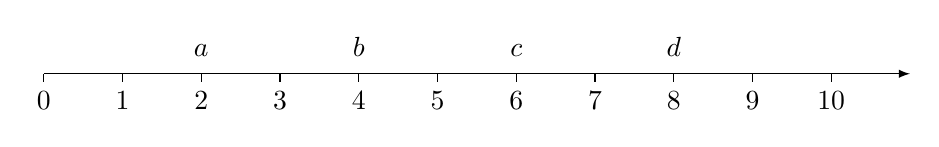
\begin{tikzpicture}
    \draw[-latex] (0,0) -- (11,0);
    \foreach \x in {0,...,10}
        \draw (\x,0) -- (\x,-3pt);
    \foreach \x in {0,...,10}
        \node [below] at (\x,-0.1) {$\x$};
    \foreach \x\y in {2/a,4/b,6/c,8/d}
        \node [above] at (\x,0.1) {$\y$};
\end{tikzpicture}
\]

The relationship between $P$ and $Q$ can then be described as 

Sadly, life is never easy. It would be perfectly agreeable if nature chose to let each ordinal measuring instrument correspond to 

\begin{framed}
    Questions for assumption two:
    \begin{itemize}
        \item How depressed are you when you are asleep?
        \item How agreeable are you when you are very focused on something?
    \end{itemize}
\end{framed}

Third, we assume that those psychological processes which are part of Q are time-dependent. These measures are shaped by different forces and the previous states of the construct \citep{olthofComplexityPsychologicalSelfratings2020b}. Their values are continuous and are related to each other in a structured manner \citep{bokerConsequencesContinuityHunt2002}. We also assume that their values are differentiable over time, changing smoothly. Their values can drop or increase very quickly, but not instantaneously. They are `complex' measures, meaning that they come to be through the interdependencies of the numerous non-trivially interacting forces that influence the system \citep{olthofComplexityTheoryPsychopathology2023}. This allows us 

The last assumption is that ordinal likert-type scales are approximations of this underlying continuous measure \citep{haslbeckRecoveringWithinpersonDynamics2022}. We cannot measure the underlying immediately, because we have to rely on . This means that if a person

\begin{framed}
    Questions for assumption four:
    \begin{itemize}
        \item Did you ever feel there were not enough answering options to answer a likert-type questionnaire fully? (Did you ever feel a 3.5 out of five about your shopping experience?)
        \item Would you have trouble answering a question with too many (ordinal) answer options?
    \end{itemize}
\end{framed}

Likert-type scales were not initially envisioned as mappings, and do not just include the 5-point scale we are all familiar with. Treating the 

The overarching goal is to model errors in . While full recovery of trajectory is impossible, it may be possible to recover some relevant aspects of the system under study. The research question is `Given that a psychological construct has a real-valued continuous trajectory, can we recover elements of it using RQA from limited sampling occurrences on an ordinal scale?'. The major elements to be examined include the stability of several recurrence indicators under degradation, the implications for measurement and analysis of time series of latent variable constructs, and the weaknesses and oversights that we found when we tried to simulate a theoretical trajectory and degrade it.  

A strength of this project is that it explicates normally tacit assumptions, and uses these assumptions to model the entire process: we model the underlying trajectory, the latent variable that estimates this trajectory, and we make an explicit prediction for its relationship if these assumptions are met. We use computational methods to generate the data because it is impossible to answer this question in the same way empirically as the real underlying trajectory is unknown. There is, however, an important trade-off being made: because we simulate our data, many of the complicating aspects that would come up during empirical studies are overlooked. We do not use real data, and that means that the inferences are only correct when our assumptions are correct. Serious objections to these assumptions can be found in the discussion section. Another weakness is that the performance of recurrence methods can be sensitive to the parameter settings of the computational model. In the current project, we treat only four different trajectories.

\section{Materials and methods}
\subsection{Stage 1: Data generation}
In the first stage, we used a toy model to simulate the data based on the \textit{3 + 1 Dimensions Model} introduced by \citep{gauldDynamicalSystemsComputational2023}. This model captures clinical observations found in psychiatric symptomatology by modeling internal factors ($y$), environmental noise ($z$), temporal specificities ($f$), and symptomatology ($x$) using coupled differential equations. $x$ is the basis of the time series. The original aim of this toy model is to simulate the trajectory of symptomatology of psychiatric symptoms over time. It is suitable for our project because the model creates realistic looking trajectories for psychological phenomena. The model uses four coupled differential equations to model the effect of time on symptom intensity. Symptom intensity is a subset of latent constructs, and we see its behaviour over time as similar to other latent constructs. It is of note that many different systems could have let to similar results to the ones outputted here. The data generating process is of secondary importance: it should result in somewhat plausible trajectories. We chose this model over more traditional choices, such as the Lorenz attractor, because we prioritized its flexibility in capturing realistic trajectories based on latent variable constructs in the social sciences.

\subsubsection{Symptom intensity}
\begin{equation}
    \tau_{x}\frac{dx}{dt} = \frac{S_{\max}}{1+\exp(\frac{Rs-y}{\lambda_{s}})} - x
\end{equation}

\subsubsection{Modelling of internal elements}
\begin{equation}
    \tau_{y}\frac{dy}{dt} = \frac{P}{1+\exp(\frac{R_{b}-y}{\lambda_{b}})} + L - xy - z
\end{equation}

\subsubsection{Modelling of perceived environment}
\begin{equation}
    \tau_{z}\frac{dz}{dt} = S(ax + \beta y)\ \zeta(t) - z
\end{equation}

\subsubsection{Temporal specificities}
\begin{equation}
    \tau_f\frac{df}{dt} = y - \lambda_f f
\end{equation}

\paragraph{Parameter definitions}
Parameter definitions and parameter settings are shortly mentioned here. For a more in-depth treatment, see Gauld and Depannemaecker \citep{gauldDynamicalSystemsComputational2023}. $\alpha$ \& $\beta$ are the weight of the effect of variables $x$ and $y$ on environmental perception. $\tau_{x,y,z,f}$ are the different time scales the equations operate on. $S_{\max}$ is the maximum level of the symptoms. $R_{s, b}$ is the sensitivity to triggering the system.  $\lambda_{s,b}$ are the slopes of the internal and symptom curves. $P$ is the maximal rate of internal elements of the systems. $S$ is the overall sensitivity to the environment. $L$ is the level of predisposing factors. $\lambda_{f}$ is the scaling factor of the slow evolution of fluctuations affecting $L$. $\zeta(t)$ is a point in the normal distribution where $\sigma = 0.5$. It is calculated at each $0.01t$, and is clamped between -1 and 1. 

\paragraph{Parameter settings}
There are four initial parameter settings that we have taken from the same source \citep{gauldDynamicalSystemsComputational2023}. They represent four different disorders. Their initial conditions are given at page~\pageref{tab:1}. Each time series is representative of a different kind of chaotic behaviour. The time series of the `healthy'-trajectory moves randomly around $0.1$. The time series of the `schizophrenia' time series moves close to 8, before dropping for intervals. Both `bereavement' and `bipolar' oscillate quickly in symptom strength, covering the full total range. For visualizations, see page~\pageref{fig:1}. 

\subsubsection{Solvers}
We used the Tsitouras 5/4 Runge-Kutta method as the solver for the differential equations, as implemented in the DifferentialEquations.jl package \citep{tsitourasRungeKuttaPairs2011}. We used standard settings for all of the parameters, aside from a higher number of maximum iterations ($1e^{7}$). The baseline is calculated for $0.01t$, where $t$ represents one day in the model. 

\subsection{Stage 2: Binning data and removing time points}
Afterwards, we systematically reduced the quality of the data. We binned the range of the width of the data into $n$ intervals of equal length, where $n$ stands for the number of bins. Moreover, we removed time points from the data by keeping the first and every $k^{th}$ observation of the simulated data.
We systematically decreased the number of bins and the number of time points, and re-analyze the data. $k$ at 1 is set at the baseline. This implies no reduction. The other $k$-values include 2, 4, and 8. For binning, $n$ = 100 is set at the baseline, and is equivalent to a visual analog scale. Other $n$-values include 20, 7, 6, 5, 4, 3, and 2. These were chosen to reflect different types of measuring instruments, such as several types of likert and forced-choice scales.

\subsection{Stage 3: Data analysis}
We judged the sensitivity of the data by deriving the recurrence indicators introduced before for each time series in each state of degradation. We calculated the deviation of each of these values from the baseline, which are the recurrence values derived for the intact dataset. We mapped the changes as the deviation for these indicators between the baseline and a set of degraded data, adjusting indicators based on line length by multiplying them by the reduction factor.

\subsubsection{Recurrence Quantification Analysis}
RQA is a method that is based on the identification of recurrent points in a time series. A point recurs if it is within the recurrence threshold of another point in time \citep{webber2005recurrence}. Indicators can then be derived from this matrix. The development of these indicators has seen considerable development \citep{marwanTrendsRecurrenceAnalysis2023}. We chose to focus on the core set of indicators, as described by Marwan and Webber \citep{marwanMathematicalComputationalFoundations2015}. The recurrence threshold was set at the size of the bins of the degraded data set. E.g., if the range of the trajectory was 0 to 2, and the number of bins is 7 (data is degraded so that it is similar to likert-scale data), then the recurrence threshold would have been set at $\frac{2-0}{7}$ = $\frac{2}{7}$. A visualization of these recurrences for the four trajectories can be found on page~\pageref{fig:2}.

\subsubsection{Recurrence Indicators}
The \textit{recurrence rate} is the proportion of points in the phase space that reoccur at later times \citep{webber2005recurrence}. Higher recurrence rates indicate that an underlying function is more periodic.\ \textit{Determinism} is the share of recurrent points that are part of diagonal lines, which indicate that the structure might be deterministic. It should be noted that it is a necessary condition, not sufficient by itself, to indicate determinism \citep{marwanHowAvoidPotential2011}.\ \textit{Average and maximum length of diagonal structures} are also given. A longer average length means more predictable dynamics. A longer maximum indicates the longest segment.\ \textit{Entropy of diagonal structures} concerns the Shannon entropy of diagonal line lengths \citep{kraemerRecurrenceThresholdSelection2018}. It is an indicator of the amount of randomness, or information, in the data.\ \textit{Trapping time} is the average length of vertical lines in the plot. It is a measure of how long a system stays in a particular state.\ \textit{Most probable recurrence time}, similarly, is the mode of the length of the vertical lines in the plot. 

\subsection{Software}
We used the Julia language, and in particular the `DynamicalSystems.jl', `RecurrenceAnalysis.jl', and `Statistics.jl' packages to implement the toy model and run the recurrence analyses \citep{bezanson2017julia, Datseris2018, DatserisParlitz2022}. Analyses were run on a personal computer. Full information about dependencies and version numbers can be found in a machine-readable format in the Manifest.toml file in the Github-repository. Instructions for running the analysis through a sandboxed project environment identical to our system can be found on the main page of this repository.

% For Original Research articles, please note that the Material and Methods section can be placed in any of the following ways: before Results, before Discussion or after Discussion.

\section{Discussion}

The Romanian economist and mathematician Georgescu-Roegen has played a similar role of aligning 

%%Figures, tables, and images will be published under a Creative Commons CC-BY licence and permission must be obtained for use of copyrighted material from other sources (including re-published/adapted/modified/partial figures and images from the internet). It is the responsibility of the authors to acquire the licenses, to follow any citation instructions requested by third-party rights holders, and cover any supplementary charges.

\section*{Conflict of Interest Statement}
The authors declare that the research was conducted in the absence of any commercial or financial relationships that could be construed as a potential conflict of interest.

\section*{Funding}
No external funding was used for this project.

\section*{Acknowledgments}
I acknowledge the work of my thesis supervisors, who introduced me to the method and left me free to pursue the project as I imagined it. The great help of the Julia community was also appreciated, as they have been pushing me forward where I got stuck and took the time to respond to my stupid questions. Finally, I would like to acknowledge the feedback and conversations between me and my thesis group, who have been working through my text and made sure that it is easy to follow and well-written. Special thanks to Giuliana Orizzonte, Daniel Anadria, dr. Derksen, and dr. Bringmann for fruitful discussions and feedback about my topic. Lastly, I would like to thank my girlfriend, family, and friends for the mental support throughout.

\section*{Data Availability Statement}
The code, additional material, and generated data for this study can be found on \href{https://github.com/MvanSteenbergen/MasterThesisRQA}{GitHub}.

% Please see the availability of data guidelines for more information, at https://www.frontiersin.org/about/author-guidelines#AvailabilityofData

\bibliographystyle{Frontiers-Harvard} %  Many Frontiers journals use the Harvard referencing system (Author-date), to find the style and resources for the journal you are submitting to: https://zendesk.frontiersin.org/hc/en-us/articles/360017860337-Frontiers-Reference-Styles-by-Journal. For Humanities and Social Sciences articles please include page numbers in the in-text citations 
%\bibliographystyle{Frontiers-Vancouver} % Many Frontiers journals use the numbered referencing system, to find the style and resources for the journal you are submitting to: https://zendesk.frontiersin.org/hc/en-us/articles/360017860337-Frontiers-Reference-Styles-by-Journal
\newpage
\bibliography{bibliography}
\newpage
\section*{Figures}
\begin{figure}[H]
    \begin{center}
    \includegraphics[width=15cm]{time_series_plot}
    \end{center}
    \caption{A section of the time series created using the coupled differential equations and parameter settings specified in section 2.1.1. This is the intact data, before degradation takes place.}\label{fig:1}
    \end{figure}

\newpage
\begin{figure}[H]
    \begin{center}
    \includegraphics[width=15cm]{recurrence_plots}
    \end{center}
    \caption{Recurrence plot for the four time series generated using the coupled differential equations and parameter settings specified in section 2.1.1. A point recurs when it is within the recurrence threshold of another point. Recurrent points are black, non-recurrent points are white. The axes represent time points, each location on the matrix represents a combination of time points. The recurrence threshold is set at 0.2 for illustration purpose. Note that the plot for the `healthy' trajectory is completely black: this is because every point in the plot falls within the recurrence threshold. Also note the black `boxes' where the bottom two trajectories are stagnant.}\label{fig:2}
    \end{figure}

\newpage
\section*{Tables}
\begin{table}[H]
    \begin{tabular}{|l| c c c c c c c c c c c c c c c|}
    \hline
    \bf{Parameter} & $S_{max}$ & $R_{s}$ & $\lambda_{s}$ & $\tau_{x}$ & $P$ & $R_{b}$ & $\lambda_{b}$ & $L$ & $\tau_{y}$ & $S$ & $\alpha$ & $\beta$ & $\tau_{z}$ & $\lambda_{d}$ & $\tau_{f}$ \\
    \hline
    \it{Healthy} & 10 & 1 & 0.1 & 14 & 10 & 1.04 & 0.05 & 0.2 & 14 & 4 & 0.5 & 0.5 & 1 & 1 & 720 \\
    \hline
    \it{Schizophrenia} & 10 & 1 & 0.1 & 14 & 10 & 0.904 & 0.05 & 0.2 & 14 & 4 & 0.5 & 0.5 & 1 & 1 & 720 \\
    \hline
    \it{Bipolar} & 10 & 1 & 0.1 & 14 & 10 & 1.04 & 0.05 & 1.01 & 14 & 10 & 0.5 & 0.5 & 1 & 1 & 720 \\
    \hline
    \it{Bereavement} & 10 & 1 & 0.1 & 14 & 10 & 1 & 0.05 & 0.6 & 14 & 4.5 & 0.5 & 0.5 & 1 & 1 & 720 \\
    \hline
    \end{tabular}
    \caption{The parameter settings used as initial parameter settings for the coupled differential equations specified in paragraph 2.1.1}\label{tab:1}
    \end{table}



    
%%% Make sure to upload the bib file along with the tex file and PDF
%%% Please see the test.bib file for some examples of references

%%% Please be aware that for original research articles we only permit a combined number of 15 figures and tables, one figure with multiple subfigures will count as only one figure.
%%% Use this if adding the figures directly in the mansucript, if so, please remember to also upload the files when submitting your article
%%% There is no need for adding the file termination, as long as you indicate where the file is saved. In the examples below the files (logo1.eps and logos.eps) are in the Frontiers LaTeX folder
%%% If using *.tif files convert them to .jpg or .png
%%%  NB logo1.eps is required in the path in order to correctly compile front page header %%%


%%% If you don't add the figures in the LaTeX files, please upload them when submitting the article.
%%% Frontiers will add the figures at the end of the provisional pdf automatically
%%% The use of LaTeX coding to draw Diagrams/Figures/Structures should be avoided. They should be external callouts including graphics.

\end{document}